\documentclass{scrartcl}
\usepackage{datatool}
\usepackage{pgffor}

\usepackage{float}
\usepackage{datatool}
\usepackage[utf8]{inputenc}
\usepackage{lmodern}
\usepackage[T1]{fontenc}
\usepackage{mathtools}
\usepackage{amssymb}
\usepackage{listings}
\usepackage{color}
\usepackage{geometry}
 \geometry{
 a4paper,
 total={170mm,257mm},
 left=20mm,
 top=20mm,
 }
\lstdefinestyle{mystyle}{
    backgroundcolor=\color{backcolour},   
    commentstyle=\color{codegreen},
    keywordstyle=\color{codeblue},
    numberstyle=\tiny\color{codegray},
    stringstyle=\color{codepurple},
    basicstyle=\footnotesize,
    breakatwhitespace=false,         
    breaklines=true,                 
    captionpos=b,                    
    keepspaces=true,                 
    numbers=left,                    
    numbersep=5pt,                  
    showspaces=false,                
    showstringspaces=false,
    showtabs=false,                  
    tabsize=2
}

\definecolor{codegreen}{rgb}{0,0.6,0}
\definecolor{codeblue}{rgb}{0,0,0.6}
\definecolor{codegray}{rgb}{0.5,0.5,0.5}
\definecolor{codepurple}{rgb}{0.58,0,0.82}
\definecolor{backcolour}{rgb}{0.95,0.95,0.92}

\usepackage{graphicx}
\graphicspath{ {img/}{img/figures/} {img/tables/}}
\newcommand\tab[1][1cm]{\hspace*{#1}}
\lstset{style=mystyle}

\title{Sprawozdanie 1 \\ Przetwarzanie równoległe}
\subtitle{Mnożenie macierzy porównanie efektywności metod –\\
3 pętle - kolejność pętli: jki,\\
6 pętli - kolejność pętli: zewnętrznych ijk, wewnętrznych: ikj, podział pracy przed pętlą 1.}
\date{2018-05-13}
\author{Bartosz Nawrotek, Krystian Hoczkiewicz \\
Prowadzący: dr inż. Rafał Walkowiak}

\begin{document}
\maketitle
\section{Wstęp}
\paragraph{}Celem sprawozdania jest analiza wraz z porównaniem efektywności dwóch metod mnożenia macierzy w wersji równoległej oraz sekwencyjnej:
\begin{itemize}
\item {3 pętle w kolejności jki}
\item {6 pętli w kolejności zewnętrznych ijk, wewnętrznych ikj z podziałem pracy przed pierwszą pętlą}
\end{itemize}
\paragraph{}Wynikiem mnożenia jest macierz $R$, czynnikami macierze $A, B$. Iloczyn jest liczony wg poniższego wzoru:
\begin{equation}
R_{i, j} = \sum_{k = 1}^{n}{A_{i, k}B_{k, j}}
\end{equation}
gdzie $n$ jest ilością wierszy macierzy kwadratowych $A$ oraz $B$.
Do przeprowadzenia pomiarów korzystano z oprogramowania Vtune oraz do pomiaru czasu działania algorytmu biblioteka <chrono>.
\subsection{System obliczeniowy}
\begin{table}[H]
\begin{tabular}{|l|l|}
\hline
Model procesora                & Intel® Xeon® Processor E3-1220 v2                       \\ \hline
Liczba rdzeni                  & 4                                                       \\ \hline
Liczba wątków                  & 4                                                       \\ \hline
Bazowa częstotliwość procesora & 3,10 GHz                                                \\ \hline
Wielkość Cache                 & 8 MB                                                    \\ \hline
Szybkość magistrali            & 5 GT/s DMI                                              \\ \hline
Pamięć operacyjna              & 12 GB DDR3 1600                                         \\ \hline
Hyper-Threading                & Brak                                                    \\ \hline
Generacja                      & Sandy Bridge                                            \\ \hline
Zestaw instrukcji              & 64-bit                                                  \\ \hline
DTBL/STBL                      & 64 wpisy adresów do 4KB stron / STBL 512 wpisów adresów \\ \hline
\end{tabular}
\end{table}
\newpage 
\section{Analiza algorytmów oraz dyrektyw Open MP}
\subsection{Metoda 3 pętlowa JKI}
\begin{lstlisting}[language=C++, caption={Metoda trzypętlowa}]
void multiply_matrices_JKI()
{
        // mnozenie macierzy 
#pragma omp parallel for 
	for (int j = 0 ; j < COLUMNS ; j++)
      	    for (int k = 0 ; k < COLUMNS ; k++) 
                  for (int i = 0 ; i < ROWS ; i++) 
                        matrix_r[i][j]+= matrix_a[i][k] * matrix_b[k][j] ;              
}
\end{lstlisting}
\paragraph{}Jak widać metoda 3 pętlowa charakteryzuje się złożonością $O(n^3)$, gdzie $COLUMNS = ROWS = n$ dla macierzy kwadratowych. W sekwencyjnej metodzie 3 pętlowej wykorzystany został ten sam kod wraz z wyłączoną obsługą dyrektyw OpenMP. W wersji równoległej następuje przydział pracy przed pierwszą pętlą. Powoduje to statyczny podział pracy wg następującego wzoru:
\begin{equation}
j = <id \frac{COLUMNS}{4}, (id + 1)\frac{COLUMNS}{4} - 1>,
j \in \mathbb{Z}
\end{equation}
gdzie $j$ oznacza numer przydzielonej iteracji do procesora o numerze $id \in \{0, 1, 2, 3\}$ dla COLUMNS podzielnego na 4.
\subsection{Metoda 6 pętlowa IJK-IKJ}
\begin{lstlisting}[language=C++, caption={Metoda sześciopętlowa}]
void multiply_matrices_IJK_IKJ()
{
	int r = 10;
	#pragma omp parallel for
	for (int i = 0; i < ROWS; i+=r) {
		for (int j = 0; j < COLUMNS; j+=r) {
			for (int k = 0; k < COLUMNS; k+=r) {
				for (int ii = i; ii < i + r; ii++) {
					for (int kk = k; kk < k + r; kk++) {
						for (int jj = j; jj < j + r; jj++) {
						matrix_r[ii][jj] += matrix_a[ii][kk] * matrix_b[kk][jj];
						}
					}
				}
			}
		}
	}
}
\end{lstlisting}
\paragraph{}Metoda 6 pętlowa wykazuje się tą samą złożonością obliczeniową co metoda 3 pętlowa. Wykorzystanie jej ma jednak wpływ na prędkość przetwarzania ze względu na budowę systemu obliczeniowego. Korzysta on z pamięci cache oraz bufora translacji, które aby optymalnie wykorzystać, należy zapewnić odpowiednie warunki przetwarzania, jak lokalność przestrzenna oraz czasowa.
\subsection{Analiza poprawności algorytmów}
\paragraph{}Oba algorytmy w wersji sekwencyjnej są poprawne, ze względu na definicję mnożenia macierzy. W wersji równoległej również, ze względu na to, że każdy proces korzysta z innej, rozłącznej części macierzy wynikowej. Nie jest wymagana żadna dodatkowa metoda synchronizacji. Nie występuje zjawisko wyściugu w dostępie.
\subsection{Efektywność - synchronizacja}
\paragraph{}Jak było nadmienione w punkcie 2.1 oraz 2.2, obie metody cechują się tą samą złożonością obliczeniową. Jednak różnice efektywności mogą być znaczne ze względu na kolejność dostępu do danych z poszczególnych macierzy. Spodziewamy się prawie 4 krotnego przyspieszenia przetwarzania przy użyciu metod w wersji równoległej w stosunku do wersji sekwencyjnej ze względu na niski koszt synchronizacji (przydział pracy statyczny przed pętlą zewnętrzną oraz synchronizacja na końcu działania funkcji).
\subsection{False sharing}
\paragraph{}Jest to zjawisko, które może wystąpić tylko w przypadku przetwarzania równoległego. W metodzie równoległej 3 pętlowej zjawisko może wystąpić na krańcach przydzielonych obszarów macierzy $R$. Nie powinno jednak mieć to większego wpływu na czas przetwarzania ze względu na stosunkowo niewielkie fragmenty macierzy, gdzie zjawisko ma możliwość się pojawić.
W metodzie równoległej 6 pętlowej zjawisko również może wystąpić na granicy ostatniego wiersza przydzielonego do danego procesora oraz pierwszego wiersza przydzielonego do kolejnego procesora. W tym wypadku, będzie prawdopodobnie niezauważalne, bo dla całej macierzy występują tylko 4 potencjalne miejsca wystąpienia tego zjawiska niezależnie od wielkości instancji.
\subsection{Lokalność dostępu do danych}
\paragraph{}Macierze deklarowane są jako tablice dwuwymiarowe, co implikuje przechowywanie ich w pamięci jako pojedyncza linia. Niesie to za sobą możliwość analizy lokalności dostępu do danych.
\begin{figure}[H]
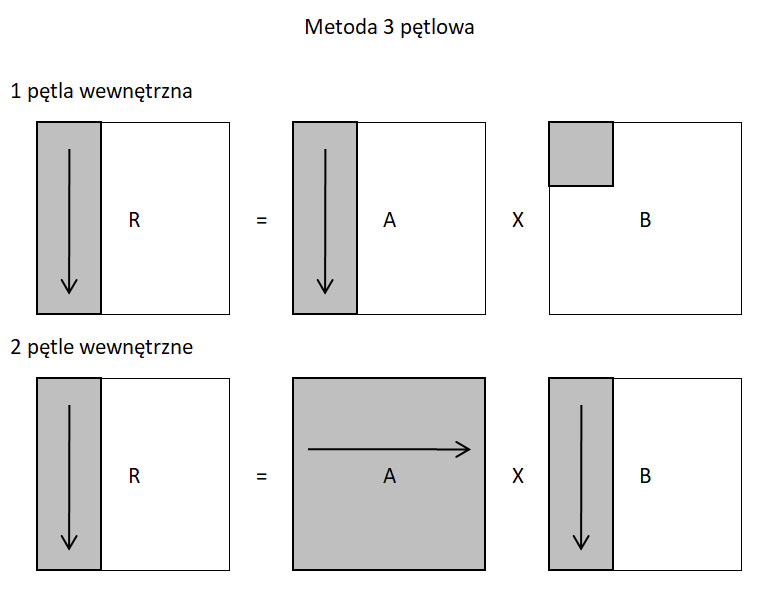
\includegraphics[width=\textwidth]{3petlowa.png}
\caption{Metoda 3 pętlowa - diagram przedstawiający korzystanie z części macierzy w kolejnych pętlach wewnętrznych}
\end{figure}
\paragraph{}Dla metody 3 pętlowej biorąc pod uwagę iteracje wewnętrznej pętli można wyciągnąć następujące wnioski dla poszczególnych macierzy: \\
\begin{itemize}
\item R - brak lokalności przestrzennej ani czasowej
\item A - brak lokalności przestrzennej ani czasowej
\item B - lokalność czasowa
\end{itemize}
\paragraph{}Natomiast dla dwóch pętli wewnętrznych:
\begin{itemize}
\item R - brak lokalności przestrzennej ani czasowej
\item A - lokalność przestrzenna, brak lokalności czasowej ze względu na odczyt danych w poszczególnych kolumnach. (kolejne czytane komórki mają oddalone adresy o $n$)
\item B - brak lokalności przestrzennej ani czasowej
\end{itemize}
\paragraph{}Braki lokalności spowodowane są iterowaniem po kolejnych elementach w kolumnach poszczególnych macierzy. Powodować to będzie znaczne spadki efektywności działania algorytm.
\subsection{Uzasadnienie wielkości instancji} Dla poprawności wzorów przyjęto wielkości instancji oraz rozmiary podmacierzy jako wielokrotności linii pamięci. 
\paragraph{Lokalność czasowa, metoda 3 pętlowa.}Aby zapewnić lokalność czasową przetwarzania należy spełnić poniższy warunek:
\begin{equation}
3 * 4N ^ 2 <= 8388608 [B]
\end{equation}
\paragraph{}Lewa strona wynika z rozmiaru trzech macierzy. Prawa strona natomiast jest rozmiarem pamięci podręcznej 8MB. Z czego mamy:
\begin{equation}
N < 837
\end{equation}
\paragraph{}Dla dwóch wewnętrznych pętli natomiast:
\begin{equation}
4N^2 + 4 * 64N \leq 8388608 [B]
\end{equation}
\paragraph{}Co daje:
\begin{equation}
N < 1417
\end{equation}
\paragraph{}Pierwszy człon jest wielkością potrzebną do zachowania macierzy $A$ w pamięci, kolejny wynika z konieczności przetrzymywania poszczególnych kolumn macierzy $R$ oraz $B$.
\paragraph{Lokalność przestrzenna}Aby zapewnić lokalność przestrzenną zdefiniowaną jako zapewnienie jednokrotnego uzupełnienia odwzorowania strony na ramkę pamięci dla $N > W_{ram}$, gdzie $W_{ram}$ jest wielkością ramki pamięci należy spełnić następujący warunek:
\begin{equation}
3*4N ^ 2 <= 576 * 4096 [B]
\end{equation}
\paragraph{}Lewa strona wynika z wielkości trzech macierzy Powyższa suma powinna mieścić się w buforze translacji o wielkości $576 * 4096[B]$. Z czego mamy:
\begin{equation}
N < 443
\end{equation}
\begin{figure}[H]
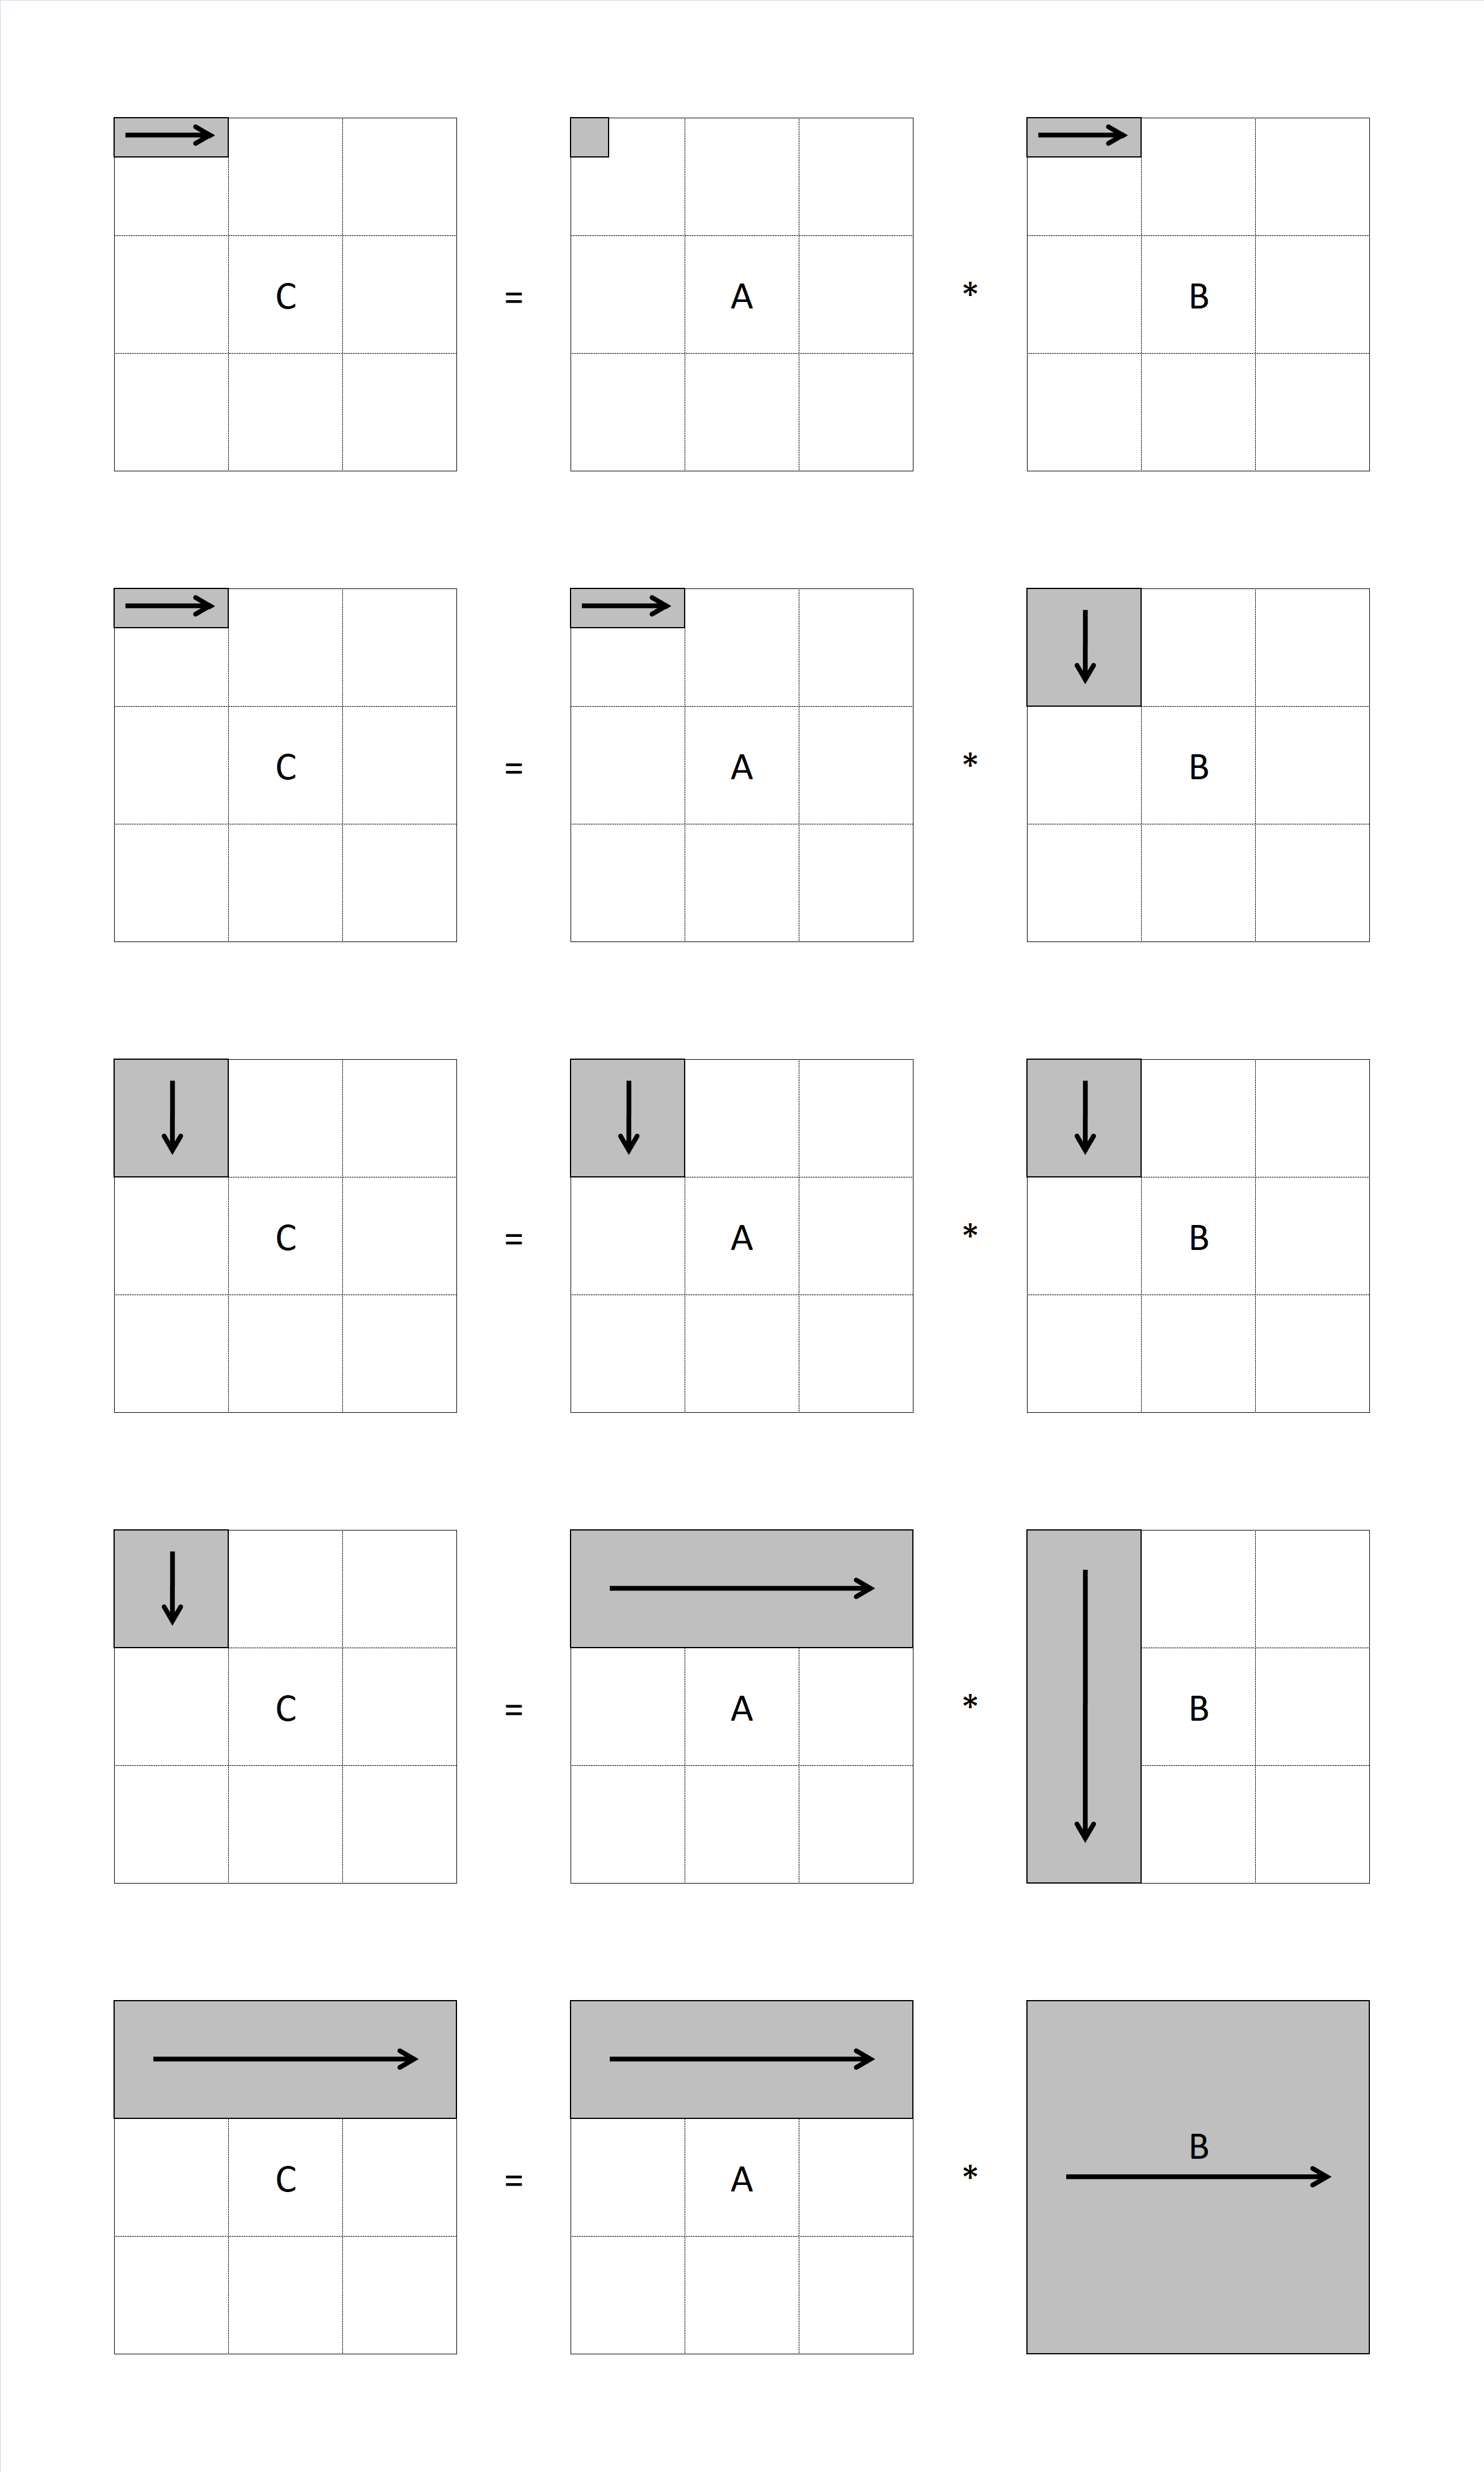
\includegraphics[width=0.9\textwidth]{6petlowa.png}
\caption{Metoda 6-cio pętlowa - diagram przedstawiający korzystanie z części macierzy w kolejnych pętlach wewnętrznych}
\end{figure}
\paragraph{}Analiza lokalności w poszczególnych zagnieżdżonych pętlach analogiczna do metody 3 pętlowej.
\paragraph{Lokalność czasowa w metodzie 6-cio pętlowej} Aby zachować lokalność czasową odwołań w przypadku metody 6-cio pętlowej należy zmieścić w pamięci podręcznej 3 podmacierze. dla każdego z wątków Z czego mamy:
\begin{equation}
r^2 * 4 * 3 \leq 8388608
\end{equation}
\paragraph{}Co daje:
\begin{equation}
r < 837
\end{equation}
\paragraph{}Niestety nie dokonano pomiarów dla tak wysokiej wartości parametru r, ponieważ na komputerze w trakcie wykonywania pomiarów działało znacznie więcej procesów, przez co udało się osiągnąć stosunkowo wysoki współczynik braku trafień już dla rozmiaru $r = 512$.
\paragraph{}Dla algorytmu w wersji sekwencyjnej mamy:
\begin{equation}
r < 1674
\end{equation}
\paragraph{}Co wymagałoby mierzenia jeszcze większych rozmiarów instancji.
\subsection{Przydział pracy do wątków}
\paragraph{}Użycie dyrektywy Open MP "\#pragma omp parallel for" sprawia, że przydział pracy do wątków jest równomierny jeżeli jest to możliwe. Taki przydział występuje gdy liczba iteracji jest podzielna przez liczbę procesorów. W przeciwnym wypadku pozostałe iteracje (ich ilość jest równa reszcie z dzielenia liczby iteracji na liczbę procesorów)jest rozdzielana między wątkami. W tym wypadku możliwe jest zaobserwowanie nieznacznego spadku efektywności działającego algorytmu, jednak sprawozdanie nie zawiera dokładnej analizy tego zjawiska.
\paragraph{}W metodzie 3 pętlowej do poszczególnych wątków przydzielanę są kolejne grupy kolumn macierzy $R$, $B$ oraz cała macierz $A$. Natomiast w metodzie 6-cio pętlowej przydzielane są grupy wierszy macierzy $C$, $A$ oraz cała macierz $B$.
\paragraph{Czas obliczeń.} Na poniższym wykresie widać zależność między czasem obliczeń, a rozmiarem instancji. Potwierdza to złożoność zaproponowanego algorytmu równą $O(n^{3})$. W dodatku różnice czasów wykonań metody sekwencyjnej oraz równoległej pokazują, że dla małych instancji problemu zastosowanie algorytmu równoległego nie musi być odpowiednie, jednak możliwości algorytmów równoległych uwidaczniają się przy większych rozmiarach instancji.
\begin{figure}[H]
\includegraphics{Tobl3.png}\\
\end{figure}
\paragraph{Prędkość obliczeń.} Wykres prędkości obliczeń w metodzie 3 pętlowej świadczy natomiast o spadku efektywności zastosowanego algorytmu dla kolejnych rozmiarów instancji w obu metodach. Powody spadku efektywnosci zostaną wymienione w dalszej części sprawozdania.
\begin{figure}[H]
\includegraphics{Predkosc3.png}\\
\end{figure}
\newpage
\paragraph{Instrukcje na cykl.} Wskaźnik \textbf{IPC} oznacza średnią liczbę instrukcji kodu asemblera przypadającą na cykl pracy procesora. Jak widać, dla metody 3 pętlowej przy rozmiarach instancji od $n = 512$ następuje gwałtowny spadek wartości wskaźnika, świadczy to o obecności czynników zmniejszających efektywność, takich jak słaba przestrzenna lub czasowa lokalność dostępów do pamięci.
\begin{figure}[H]
\includegraphics{IPC3.png}\\
\end{figure}
\newpage
\paragraph{Stosunek braku trafień do L2 DTLB.} Na wykresie można zauważyć osiągnięcie stusunku braku trafień bliskiego $1$ już dla rozmiaru instancji $n = 512$, potwierdza to przewidywania dotyczące słabej lokalności przestrzennej dostępów do pamięci powyżej rozmiaru instancji $N > 443$. Implikuje to znaczny spadek efektywności przetwarzania.
\begin{figure}[H]
\includegraphics{SBTDPPL33.png}\\
\end{figure}
\newpage
\paragraph{Wskaźnik braku trafień do pp L3.} Wskaźnik został policzony wg wzoru: $PPL3\ miss\ rate = L3\ miss / Data\ access$. Dla $Data\ access = 0$ przyjęto, że wartość wskaźnika bedzie równa 0, taka sytuacja może mieć miejsce ze względu na brak przekroczenia progu zliczania przy pomiarze dla małych rozmiarów instancji. Wartosci wskaźnika wskazują na niską lokalność czasową dostępów do pamięci. Dla małych rozmiarów instancji wskaźnik ma wartość 0 ze względu na fakt, że macierze są przetrzymywane w pamięci podręcznej od chwili ich inicjalizacji.
\begin{figure}[H]
\includegraphics{L3MissRate3.png}
\end{figure}
\newpage
\paragraph{Przyspieszenie} Przyspieszenie osiąga wartość ponad $3.5$ od instancji o rozmiarze $n = 512$, świadczy to o tym, że problem jest łatwy do zrównoleglenia, nie narzuca wysokich kosztów synchronizacji, aby zachować poprawność.
\begin{figure}[H]
\includegraphics{Przyspieszenie3.png}
\end{figure}
\paragraph{Koszt synchronizacji} Koszt synchronizacji maleje wraz z rozmiarem instancji. Jest to zrozumiałe ze względu na fakt, że istnieje tylko jeden punkt synchronizacji wątków niezależnie od rozmiaru instancji.
\begin{figure}[H]
\includegraphics{Synchro3.png}
\end{figure}

\subsection{Metoda 6cio pętlowa}

\paragraph{Czas obliczeń.} Wykres czasu obliczeń w metodzie 6-cio pętlowej również wskazuje na złożoność obliczeniową problemu. Można zaobserwować również różnice w czasie obliczeń w zależności od wielkości parametru $r$. Jest ona spowodowana zajmowaniem przez kolejne podmacierze różnej ilości miejsca w pamięci podręcznej. W dalszej części sprawozdania przyjmujemy, że w nazwie instancji metody sześciopętlowej znajdują się odpowiednio $n$ oraz $r$ oddzielone separatorem '\_'
\begin{figure}[H]
\includegraphics{Tobl6.png}
\end{figure}

\newpage
\paragraph{Prędkość obliczeń.} Dla metody 6-cio pętlowej prędkość obliczeń ulega niewielkim wahaniom w zależnosci od rozmiaru instancji, co pokazuje, że zastosowanie algorytmu 6-cio pętlowego pozwala poprawić lokalność przestrzenną lub czasową dostępów. Dla metody równoległej w zależności od wielkości parametru $r$ prędkość obliczeń ulega dużej zmianie. Najlepsze wyniki zostały uzyskane dla $r = 64$, następnie wraz ze wzrostem $r$, prędkość zaczyna maleć. Jest to spowodowane utratą czasowej lokalności dostępów do pamięci ze względu na zajmowanie przez podmacierz dużej ilości miejsca w pamięci podręcznej dla kolejnych zagnieżdżeń pętli. Z drugiej jednak strony dla wielkości $r = 16$ również następuje spadek prędkości ze względu na częste odwołania do pp, przez co musi być ona częściej aktualizowana. Dla metody sekwencyjnej najlepszą mierzoną wartością r było 16, różnica może wynikać z tego, że dla wielu procesorów lokalnoś czasowa w ramach pętli czwartej wewnętrznej pozwala na wielokrotne używanie kolumny macierzy B przez wszystkie procesory.
\begin{figure}[H]
\includegraphics{Predkosc6.png}\\
\end{figure}

\newpage
\paragraph{Instrukcje na cykl.} W odróżnieniu od metody 3 pętlowej wartość wskaźnika IPC utrzymuje podobną wartość w zależności od rozmiaru instancji, co wskazuje na obniżenie wpływu czynników obniżających efektywność przetwarzania kodu.
\begin{figure}[H]
\includegraphics{IPC6.png}\\
\end{figure}

\newpage
\paragraph{Stosunek braku trafień do L2 DTLB.} Dla metody 6-cio pętlowej przy odpowiednim doborze parametru $r$ można zapewnić lokalność przestrzenną dostępu do danych. W przypadku wybranych wartości $r$ udaje się zachować lokalność przestrzenną dla $r \in \{64, 128, 256\}$. TODO
\begin{figure}[H]
\includegraphics{SBTDPPL36.png}\\
\end{figure}

\newpage
\paragraph{Wskaźnik braku trafień do pp L3.} W większości przypadków udało się utrzymać wskaźnik braku trafień do pp L3 na niskim poziomie, co wskazuje na to, że przy odpowiednim doborze parametru $r$ zachowujemy również lokalność czasową odwołań. Wyjątki widoczne na wykresie wynikają z  z częstego odwoływania się pp co może powodować częste pobieranie danych do pamięci podręcznej.
\begin{figure}[H]
\includegraphics{L3MissRate6.png}
\end{figure}

\newpage
\paragraph{Przyspieszenie} Uzyskane wyniki przyspieszenia pozwalają stwierdzić, że dla metody 6-cio pętlowej również można osiągnąć wysoki stopień zrównoleglenia Skrajnie niskie wartości przyspieszenia wynikają z braku lokalności dostępów w metodzie równoległej, przy zachowaniu lokalności w metodzie sekwencyjnej. Niestety nie zostało to pokazane na poprzednich wykresach ze względu na mały rozmiar instancji, który nie pozwalał na przekroczenie dobranego progu zliczania.
\begin{figure}[H]
\includegraphics{Przyspieszenie6.png}
\end{figure}

\newpage
\paragraph{Koszt synchronizacji} Koszt synchronizacji podobnie jak w przypadku metody 3 pętlowej maleje wraz ze wzrostem rozmiaru instancji.
\begin{figure}[H]
\includegraphics{Synchro6.png}
\end{figure}

\section{Wnioski}
\paragraph{} W sprawozdaniu udało się potwierdzić tezę o możliwości utrzymania efektywności przetwarzania niezależnie od wielkości instancji stosując metodę sześciopętlową dla problemu mnożenia macieży. Pokazuje to konieczność szerszej analizy działania algorytmów, niż tylko ograniczanie do złożoności obliczeniowej, która to w obu metodach była jednakowa. Dodatkowo pokazano, że koszty synchronizacji w obu metodach są bardzo niskie przez co problem mnożenia macierzy jest łatwy do zrównoleglenia. Ponadto porównując wykonywanie algorytmu na jednym oraz na 4 procesorach udało się pokazać, że rozwiązanie jest łatwo skalowalne, zachowany zostaje niski koszt synchronizacji, a uzyskane przyspieszenie jest prawie tylokrotne, co iloraz ilości wykorzystanych współbieżnie działających wątków. 
\section{Wyniki tabelaryczne}
\paragraph{} Poniżej zostały przedstawione wyniki tabelaryczne, na podstawie których zostały utworzone wykresy.
\begin{table}[H]
\begin{tabular}{|l|l|l|}
\hline
Wartosc wskaźnika IPC         & metoda równoległa & metoda sekwencyjna \\ \hline
multiply\_matrices\_JKI\_256  & 6.9e-01           & 6.9e-01            \\ \hline
multiply\_matrices\_JKI\_512  & 1.5e-01           & 1.3e-01            \\ \hline
multiply\_matrices\_JKI\_768  & 1.5e-01           & 1.3e-01            \\ \hline
multiply\_matrices\_JKI\_1024 & 1.5e-01           & 1.3e-01            \\ \hline
multiply\_matrices\_JKI\_1536 & 1.4e-01           & 1.3e-01            \\ \hline
multiply\_matrices\_sixLoops\_256\_16   & 2.8e+00           & 1.7e+00            \\ \hline
multiply\_matrices\_sixLoops\_256\_64   & 3.0e+00           & 3.5e+00            \\ \hline
multiply\_matrices\_sixLoops\_256\_128  & 1.8e+00           & 1.5e+00            \\ \hline
multiply\_matrices\_sixLoops\_512\_16   & 3.2e+00           & 2.3e+00            \\ \hline
multiply\_matrices\_sixLoops\_512\_64   & 2.5e+00           & 2.4e+00            \\ \hline
multiply\_matrices\_sixLoops\_512\_128  & 2.2e+00           & 2.0e+00            \\ \hline
multiply\_matrices\_sixLoops\_512\_256  & 2.0e+00           & 2.4e+00            \\ \hline
multiply\_matrices\_sixLoops\_768\_16   & 2.9e+00           & 2.1e+00            \\ \hline
multiply\_matrices\_sixLoops\_768\_64   & 2.7e+00           & 2.4e+00            \\ \hline
multiply\_matrices\_sixLoops\_768\_128  & 2.2e+00           & 2.0e+00            \\ \hline
multiply\_matrices\_sixLoops\_1024\_16  & 2.8e+00           & 1.9e+00            \\ \hline
multiply\_matrices\_sixLoops\_1024\_64  & 2.7e+00           & 2.3e+00            \\ \hline
multiply\_matrices\_sixLoops\_1024\_128 & 2.2e+00           & 1.9e+00            \\ \hline
multiply\_matrices\_sixLoops\_1024\_256 & 2.0e+00           & 2.3e+00            \\ \hline
multiply\_matrices\_sixLoops\_1024\_512 & 2.0e+00           & 2.0e+00            \\ \hline
multiply\_matrices\_sixLoops\_1536\_16  & 2.6e+00           & 1.7e+00            \\ \hline
multiply\_matrices\_sixLoops\_1536\_64  & 2.6e+00           & 2.3e+00            \\ \hline
multiply\_matrices\_sixLoops\_1536\_128 & 2.1e+00           & 1.9e+00            \\ \hline
multiply\_matrices\_sixLoops\_1536\_256 & 2.0e+00           & 2.3e+00            \\ \hline
multiply\_matrices\_sixLoops\_1536\_512 & 1.9e+00           & 2.0e+00            \\ \hline
\end{tabular}
\end{table}

\begin{table}[H]
\begin{tabular}{|l|l|l|}
\hline
Wskaźnik braku trafień do PP L3 & metoda równoległa & metoda sekwencyjna \\ \hline
multiply\_matrices\_JKI\_256    & 2.8e-03           & 0.0e+00            \\ \hline
multiply\_matrices\_JKI\_512    & 2.6e-03           & 1.0e-02            \\ \hline
multiply\_matrices\_JKI\_768    & 5.3e-03           & 2.2e-02            \\ \hline
multiply\_matrices\_JKI\_1024   & 1.3e-02           & 3.2e-02            \\ \hline
multiply\_matrices\_JKI\_1536   & 2.1e-02           & 3.1e-02            \\ 
\hline
multiply\_matrices\_sixLoops\_256\_16   & 0.0e+00           & 0.0e+00            \\ \hline
multiply\_matrices\_sixLoops\_256\_64   & 0.0e+00           & 0.0e+00            \\ \hline
multiply\_matrices\_sixLoops\_256\_128  & 0.0e+00           & 1.3e-02            \\ \hline
multiply\_matrices\_sixLoops\_512\_16   & 0.0e+00           & 0.0e+00            \\ \hline
multiply\_matrices\_sixLoops\_512\_64   & 0.0e+00           & 3.0e-03            \\ \hline
multiply\_matrices\_sixLoops\_512\_128  & 0.0e+00           & 0.0e+00            \\ \hline
multiply\_matrices\_sixLoops\_512\_256  & 0.0e+00           & 0.0e+00            \\ \hline
multiply\_matrices\_sixLoops\_768\_16   & 0.0e+00           & 7.1e-04            \\ \hline
multiply\_matrices\_sixLoops\_768\_64   & 0.0e+00           & 1.3e-03            \\ \hline
multiply\_matrices\_sixLoops\_768\_128  & 0.0e+00           & 4.2e-04            \\ \hline
multiply\_matrices\_sixLoops\_1024\_16  & 3.2e-04           & 3.4e-03            \\ \hline
multiply\_matrices\_sixLoops\_1024\_64  & 1.8e-04           & 1.4e-03            \\ \hline
multiply\_matrices\_sixLoops\_1024\_128 & 3.6e-04           & 1.8e-04            \\ \hline
multiply\_matrices\_sixLoops\_1024\_256 & 5.6e-04           & 3.8e-04            \\ \hline
multiply\_matrices\_sixLoops\_1024\_512 & 0.0e+00           & 1.9e-04            \\ \hline
multiply\_matrices\_sixLoops\_1536\_16  & 1.5e-03           & 7.9e-03            \\ \hline
multiply\_matrices\_sixLoops\_1536\_64  & 6.4e-04           & 1.2e-03            \\ \hline
multiply\_matrices\_sixLoops\_1536\_128 & 2.2e-04           & 3.8e-04            \\ \hline
multiply\_matrices\_sixLoops\_1536\_256 & 3.3e-04           & 1.6e-04            \\ \hline
multiply\_matrices\_sixLoops\_1536\_512 & 6.6e-04           & 5.0e-04            \\ \hline
\end{tabular}
\end{table}

\begin{table}[H]
\begin{tabular}{|l|l|l|}
\hline
Średnia prędkość obliczeń{[}GFLOPS{]} & metoda równoległa & metoda sekwencyjna \\ \hline
multiply\_matrices\_JKI\_256          & 1.4e+00           & 5.6e-01            \\ \hline
multiply\_matrices\_JKI\_512          & 4.2e-01           & 1.2e-01            \\ \hline
multiply\_matrices\_JKI\_768          & 4.3e-01           & 1.2e-01            \\ \hline
multiply\_matrices\_JKI\_1024         & 4.4e-01           & 1.2e-01            \\ \hline
multiply\_matrices\_JKI\_1536         & 4.3e-01           & 1.2e-01            \\ \hline
multiply\_matrices\_sixLoops\_256\_16   & 2.0e+01           & 1.6e+01            \\ \hline
multiply\_matrices\_sixLoops\_256\_64   & 2.0e+01           & 1.1e+01            \\ \hline
multiply\_matrices\_sixLoops\_256\_128  & 2.0e+01           & 9.7e+00            \\ \hline
multiply\_matrices\_sixLoops\_512\_16   & 2.9e+01           & 1.5e+01            \\ \hline
multiply\_matrices\_sixLoops\_512\_64   & 4.1e+01           & 1.1e+01            \\ \hline
multiply\_matrices\_sixLoops\_512\_128  & 2.8e+01           & 9.9e+00            \\ \hline
multiply\_matrices\_sixLoops\_512\_256  & 1.7e+01           & 8.5e+00            \\ \hline
multiply\_matrices\_sixLoops\_768\_16   & 2.7e+01           & 1.4e+01            \\ \hline
multiply\_matrices\_sixLoops\_768\_64   & 3.7e+01           & 1.1e+01            \\ \hline
multiply\_matrices\_sixLoops\_768\_128  & 2.7e+01           & 9.6e+00            \\ \hline
multiply\_matrices\_sixLoops\_1024\_16  & 2.9e+01           & 1.3e+01            \\ \hline
multiply\_matrices\_sixLoops\_1024\_64  & 3.5e+01           & 1.1e+01            \\ \hline
multiply\_matrices\_sixLoops\_1024\_128 & 3.2e+01           & 9.5e+00            \\ \hline
multiply\_matrices\_sixLoops\_1024\_256 & 3.0e+01           & 8.5e+00            \\ \hline
multiply\_matrices\_sixLoops\_1024\_512 & 1.8e+01           & 9.3e+00            \\ \hline
multiply\_matrices\_sixLoops\_1536\_16  & 2.7e+01           & 1.2e+01            \\ \hline
multiply\_matrices\_sixLoops\_1536\_64  & 3.7e+01           & 1.1e+01            \\ \hline
multiply\_matrices\_sixLoops\_1536\_128 & 3.1e+01           & 9.1e+00            \\ \hline
multiply\_matrices\_sixLoops\_1536\_256 & 2.5e+01           & 8.5e+00            \\ \hline
multiply\_matrices\_sixLoops\_1536\_512 & 2.7e+01           & 9.3e+00            \\ \hline
\end{tabular}
\end{table}

\begin{table}[H]
\begin{tabular}{|l|l|}
\hline
Przyspieszenie & 3 pętlowa \\ \hline
256            & 2.5e+00   \\ \hline
512            & 3.6e+00   \\ \hline
768            & 3.6e+00   \\ \hline
1024           & 3.6e+00   \\ \hline
1536           & 3.6e+00   \\ \hline
256\_16        & 1.2e+00       \\ \hline
256\_64        & 1.9e+00       \\ \hline
256\_128       & 2.0e+00       \\ \hline
512\_16        & 1.9e+00       \\ \hline
512\_64        & 3.7e+00       \\ \hline
512\_128       & 2.8e+00       \\ \hline
512\_256       & 2.0e+00       \\ \hline
768\_16        & 1.9e+00       \\ \hline
768\_64        & 3.4e+00       \\ \hline
768\_128       & 2.8e+00       \\ \hline
1024\_16       & 2.2e+00       \\ \hline
1024\_64       & 3.3e+00       \\ \hline
1024\_128      & 3.4e+00       \\ \hline
1024\_256      & 3.5e+00       \\ \hline
1024\_512      & 2.0e+00       \\ \hline
1536\_16       & 2.2e+00       \\ \hline
1536\_64       & 3.4e+00       \\ \hline
1536\_128      & 3.4e+00       \\ \hline
1536\_256      & 2.9e+00       \\ \hline
1536\_512      & 2.9e+00       \\ \hline
\end{tabular}
\end{table}

\begin{table}[H]
\begin{tabular}{|l|l|l|}
\hline
Stosunek braku trafień do L2 DTLB & metoda równoległa & metoda sekwencyjna \\ \hline
multiply\_matrices\_JKI\_256      & 2.1e-01           & 1.8e-01            \\ \hline
multiply\_matrices\_JKI\_512      & 9.9e-01           & 1.0e+00            \\ \hline
multiply\_matrices\_JKI\_768      & 9.8e-01           & 1.0e+00            \\ \hline
multiply\_matrices\_JKI\_1024     & 9.9e-01           & 9.9e-01            \\ \hline
multiply\_matrices\_JKI\_1536     & 9.9e-01           & 9.9e-01            \\ \hline
multiply\_matrices\_sixLoops\_256\_16   & 0.0e+00           & 0.0e+00            \\ \hline
multiply\_matrices\_sixLoops\_256\_64   & 0.0e+00           & 8.3e-02            \\ \hline
multiply\_matrices\_sixLoops\_256\_128  & 0.0e+00           & 0.0e+00            \\ \hline
multiply\_matrices\_sixLoops\_512\_16   & 6.7e-02           & 1.3e-01            \\ \hline
multiply\_matrices\_sixLoops\_512\_64   & 1.5e-02           & 1.1e-02            \\ \hline
multiply\_matrices\_sixLoops\_512\_128  & 1.5e-02           & 0.0e+00            \\ \hline
multiply\_matrices\_sixLoops\_512\_256  & 0.0e+00           & 0.0e+00            \\ \hline
multiply\_matrices\_sixLoops\_768\_16   & 1.9e-01           & 3.1e-01            \\ \hline
multiply\_matrices\_sixLoops\_768\_64   & 8.6e-03           & 1.0e-02            \\ \hline
multiply\_matrices\_sixLoops\_768\_128  & 1.3e-02           & 4.1e-03            \\ \hline
multiply\_matrices\_sixLoops\_1024\_16  & 2.0e-01           & 3.2e-01            \\ \hline
multiply\_matrices\_sixLoops\_1024\_64  & 7.3e-03           & 1.1e-02            \\ \hline
multiply\_matrices\_sixLoops\_1024\_128 & 5.7e-03           & 3.5e-03            \\ \hline
multiply\_matrices\_sixLoops\_1024\_256 & 7.2e-03           & 9.6e-03            \\ \hline
multiply\_matrices\_sixLoops\_1024\_512 & 2.9e-01           & 2.8e-01            \\ \hline
multiply\_matrices\_sixLoops\_1536\_16  & 2.2e-01           & 3.4e-01            \\ \hline
multiply\_matrices\_sixLoops\_1536\_64  & 8.7e-03           & 8.5e-03            \\ \hline
multiply\_matrices\_sixLoops\_1536\_128 & 4.1e-03           & 3.2e-03            \\ \hline
multiply\_matrices\_sixLoops\_1536\_256 & 6.5e-03           & 1.1e-02            \\ \hline
multiply\_matrices\_sixLoops\_1536\_512 & 3.0e-01           & 2.9e-01            \\ \hline
\end{tabular}
\end{table}

\begin{table}[H]
\begin{tabular}{|l|l|}
\hline
Kosz synchronizacji           & 3petlowa \\ \hline
multiply\_matrices\_JKI\_256  & 3.5e-01  \\ \hline
multiply\_matrices\_JKI\_512  & 1.3e-01  \\ \hline
multiply\_matrices\_JKI\_768  & 1.0e-01  \\ \hline
multiply\_matrices\_JKI\_1024 & 9.4e-02  \\ \hline
multiply\_matrices\_JKI\_1536 & 1.0e-01  \\ \hline
multiply\_matrices\_sixLoops\_256\_16   & 4.1e-01  \\ \hline
multiply\_matrices\_sixLoops\_256\_64   & 5.4e-01  \\ \hline
multiply\_matrices\_sixLoops\_256\_128  & 4.1e-01  \\ \hline
multiply\_matrices\_sixLoops\_512\_16   & 2.5e-01  \\ \hline
multiply\_matrices\_sixLoops\_512\_64   & 5.6e-02  \\ \hline
multiply\_matrices\_sixLoops\_512\_128  & 2.9e-01  \\ \hline
multiply\_matrices\_sixLoops\_512\_256  & 5.4e-01  \\ \hline
multiply\_matrices\_sixLoops\_768\_16   & 2.1e-01  \\ \hline
multiply\_matrices\_sixLoops\_768\_64   & 1.7e-01  \\ \hline
multiply\_matrices\_sixLoops\_768\_128  & 3.3e-01  \\ \hline
multiply\_matrices\_sixLoops\_1024\_16  & 1.4e-01  \\ \hline
multiply\_matrices\_sixLoops\_1024\_64  & 2.2e-01  \\ \hline
multiply\_matrices\_sixLoops\_1024\_128 & 1.6e-01  \\ \hline
multiply\_matrices\_sixLoops\_1024\_256 & 1.7e-01  \\ \hline
multiply\_matrices\_sixLoops\_1024\_512 & 5.1e-01  \\ \hline
multiply\_matrices\_sixLoops\_1536\_16  & 1.1e-01  \\ \hline
multiply\_matrices\_sixLoops\_1536\_64  & 1.6e-01  \\ \hline
multiply\_matrices\_sixLoops\_1536\_128 & 1.5e-01  \\ \hline
multiply\_matrices\_sixLoops\_1536\_256 & 3.2e-01  \\ \hline
multiply\_matrices\_sixLoops\_1536\_512 & 2.4e-01  \\ \hline
\end{tabular}
\end{table}

\begin{table}[H]
\begin{tabular}{|l|l|l|}
\hline
Czas obliczeń{[}s{]}               & metoda sekwencyjna & metoda równoległa \\ \hline
multiply\_seq\_matrices\_JKI\_256  & 6.0e-02            & 2.4e-02           \\ \hline
multiply\_seq\_matrices\_JKI\_512  & 2.3e+00            & 6.3e-01           \\ \hline
multiply\_seq\_matrices\_JKI\_768  & 7.6e+00            & 2.1e+00           \\ \hline
multiply\_seq\_matrices\_JKI\_1024 & 1.8e+01            & 4.9e+00           \\ \hline
multiply\_seq\_matrices\_JKI\_1536 & 6.1e+01            & 1.7e+01           \\ \hline
multiply\_seq\_matrices\_sixLoops\_256\_16   & 2.1e-03            & 1.7e-03           \\ \hline
multiply\_seq\_matrices\_sixLoops\_256\_64   & 3.1e-03            & 1.6e-03           \\ \hline
multiply\_seq\_matrices\_sixLoops\_256\_128  & 3.4e-03            & 1.7e-03           \\ \hline
multiply\_seq\_matrices\_sixLoops\_512\_16   & 1.7e-02            & 9.3e-03           \\ \hline
multiply\_seq\_matrices\_sixLoops\_512\_64   & 2.4e-02            & 6.6e-03           \\ \hline
multiply\_seq\_matrices\_sixLoops\_512\_128  & 2.7e-02            & 9.5e-03           \\ \hline
multiply\_seq\_matrices\_sixLoops\_512\_256  & 3.1e-02            & 1.6e-02           \\ \hline
multiply\_seq\_matrices\_sixLoops\_768\_16   & 6.3e-02            & 3.3e-02           \\ \hline
multiply\_seq\_matrices\_sixLoops\_768\_64   & 8.2e-02            & 2.4e-02           \\ \hline
multiply\_seq\_matrices\_sixLoops\_768\_128  & 9.5e-02            & 3.4e-02           \\ \hline
multiply\_seq\_matrices\_sixLoops\_1024\_16  & 1.6e-01            & 7.4e-02           \\ \hline
multiply\_seq\_matrices\_sixLoops\_1024\_64  & 2.0e-01            & 6.1e-02           \\ \hline
multiply\_seq\_matrices\_sixLoops\_1024\_128 & 2.3e-01            & 6.7e-02           \\ \hline
multiply\_seq\_matrices\_sixLoops\_1024\_256 & 2.5e-01            & 7.2e-02           \\ \hline
multiply\_seq\_matrices\_sixLoops\_1024\_512 & 2.3e-01            & 1.2e-01           \\ \hline
multiply\_seq\_matrices\_sixLoops\_1536\_16  & 5.9e-01            & 2.7e-01           \\ \hline
multiply\_seq\_matrices\_sixLoops\_1536\_64  & 6.8e-01            & 2.0e-01           \\ \hline
multiply\_seq\_matrices\_sixLoops\_1536\_128 & 8.0e-01            & 2.3e-01           \\ \hline
multiply\_seq\_matrices\_sixLoops\_1536\_256 & 8.5e-01            & 3.0e-01           \\ \hline
multiply\_seq\_matrices\_sixLoops\_1536\_512 & 7.8e-01            & 2.7e-01           \\ \hline
\end{tabular}
\end{table}



\end{document}